%!TEX root = ../main.tex

\subsection{Controller Area Network (CAN)}\label{sec:canbusanalysis}
The CAN protocol was originally developed in the 1980's by Bosch.
It is a multi-master network, where each node connects to a common bus.
All nodes are able to broadcast data to all other nodes.
The CAN protocol includes an overhead of 47 bit per message.
The data sent in a message can vary in size from 0 to 8 bytes.
This is described in detail in section~\ref{sub:CanMessageFrame}.
The bus offers 1 Mbit/s on a bus of up to 40 \si{\metre} of length.

\begin{figure}[h!]
	\centering
	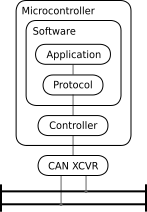
\includegraphics{graphics/canbus_setup}
	\caption{CAN node architecture}
	\label{fig:canbus_setup}
\end{figure}

Some hardware is necessary in order to properly realise a CAN network.
The structure of each node can be seen on figure~\ref{fig:canbus_setup}.
The following paragraphs explain the physical parts of this structure as well as the requirements of the protocol.

\paragraph*{The CAN Bus}~\\
The bus is shown on figure~\ref{fig:analysisnodes}.
It is a differential voltage bus.
This means that the value on the bus is determined by the voltage difference between the two wires, rather than the absolute voltage of either wire.
The bus has to be made with twisted pair wires with a characteristic impedance of $\si{120 \ohm}$ and terminated at each end with $\si{120 \ohm}$ resistors.
This increases the EMC of the bus, as inductive noise present on one wire is likely also present on the other, and the noise will then cancel itself out.

Because it's a differential bus, if the bus is broken at any point, no communication will be received, even if the receiving node still has a galvanic connection to the transmitting node.
Alternatively, it is possible to terminate each node, but this greatly reduces transmission speed.

\begin{figure}[h]
	\centering
	\includegraphics[width=.75\linewidth]{graphics/analysis_nodes}
	\caption{Overview of the network structure.}
	\label{fig:analysisnodes}
\end{figure}

\paragraph*{The CAN Transceiver (XCVR)}~\\
As CAN uses differential voltages, it is not possible to implement directly in the micro controllers.
Typically a micro controller has digital ports putting out either $ 0 \si{\volt}$, or a fixed voltage level defined as "high".
That is, depending on the voltage level, the signal is perceived as either high or low.
As mentioned above, the absolute voltage of either wire of the CAN bus does not matter, but difference in voltage does. 
As there are multiple nodes on the same bus, it is also important for one node to be able to dominate, and the other nodes to know that there is a dominant node.
The transceivers translate a voltage signal from the CAN controller (Tx) to the differential CAN signal, and simultaneously translates the bus signal to a voltage signal to the CAN controller (Rx).
That means, that while a node is sending, Tx and Rx is the same.


The transceivers monitor the bus while transmitting, to see if another node is being dominant, and if that is the case, it will start receiving data.

\paragraph*{The CAN Controller}~\\
This element can be standalone hardware, but it is in many cases built into the micro-controller.
If the CAN controller notices that the Rx it receives is not the same as the Tx it sends out, it will know that it is being dominated.
Due to the tight timing demands, this cannot be implemented in software on a chip that also needs to handle other tasks and interfaces.
The major advantage of having the controller built into the micro-controller is that it would otherwise require additional communication, like UART or SPI, for the communication between the microprocessor and controller.
A CAN controller (both standalone and built-in) has an input and output FIFO, meaning that the CAN bus communication can operate asynchronously.
This does, however, mean that it can not be used as a real time network.
Asynchronous operation is necessary as there is only one bus and it is possible that nodes will attempt to transmit messages simultaneously.

\paragraph*{Protocol}~\\
The CAN standard, apart from a variety of hardware requirements, also defines a protocol that nodes on a CAN bus should adhere to.
Part of this protocol is a well defined message frame.
A detailed description of this frame can be seen in section \ref{sub:CanMessageFrame}.\\
It should be possible to toggle the data collection of individual nodes.
This means that it is necessary to have a protocol that allows addressing each node on the bus individually.
The message frame of the CAN protocol does include a message ID, however this id holds no information about the sender of the message.
In CAN a table of all message ID's and their meaning is used to decode messages.
This table is called an object dictionary.
Achieving the desired functionality will require an adaptation of the protocol. 
\\~\\
One such adaption already exists in the form of CANopen.
CANopen is a widely used standard that builds upon CAN.
\cite{CANopen_introduction} shows that CAN accounts for the physical and data-link layers in the OSI model while CANopen accounts for the network to application layer.
It is already used in the communication with the Sevcon Gen4 and as such, using this protocol would mean that the Sevcon could be connected directly on the bus.
CANopen is quite extensive, implementing many features that are not necessarily beneficial in this application.
The many features also adds to the complexity of learning how to use the system.
It also adds a significant amount of overhead for each message, taking up bandwidth which could have otherwise been used for data. 
All of this is explored in depth in section~\ref{sub:CAN_protocol}.
\\~\\
Another option is to create a custom protocol, using CAN as the physical and data-link layers.
Designing a custom protocol means that the overhead can be reduced to the bare minimum.
This would allow for a smaller, simpler protocol.
As described in section \ref{sec:data_collection}, the protocol should support up to 16 nodes and allow for addition of new nodes.
Since it is required to toggle the data production from a node, it should also be possible to address every node individually.
